\chapter{Protocol stack implementation}
\label{chap:protocol_stack_implementation}

This chapter is dedicated to the \proj{OsmocomBB} implementation of the
\gls{gsm} \gls{ms} protocol stack. It is meant to serve as a small guide
into the source code by providing an overview of its inner workings, as
well as references to the available documentation. The information is
directly extracted from the \gls{3gpp} specifications, from the source
code, and from the project wiki. Since it would be impossible to cover
every aspect of this protocol stack in one chapter, it only provides
information relevant for the other chapters of this thesis. For more
information, refer to the specifications
directly~\cite{3gpp_specifications_????,osmocombb_ms-side_????,osmocombb_2015}.

%3GPP TS 44.001 version 12.0.0 Release 12 9 {
As explained in~\Cref{chap:network_architecture}, the \gls{ms} is
connected to the network through the Um interface, or air interface. The
protocols on this interface are separated in three layers: the physical
layer, or layer 1, the data link layer, or layer 2, and layer 3.
Each will be investigated in turn in the following
sections~\cite{3gpp_ts_2014-2}.
%}

\section{Physical layer}

  %3GPP TS 44.004 version 12.0.0 Release 12 8 {
  The first layer of the \gls{gsm} \gls{ms} protocol stack is the
  physical layer, which provides logical channels for the upper layers.
  There are two types of logical channels: channels dedicated to
  signaling data, and channels dedicated to voice traffic. The
  establishment, release, and control of the signaling channels is
  supervised by the \gls{rr} sublayer of the layer 3, based on
  measurements from layer 1. This allows the \gls{ms} to select the best
  cell, but also to adapt the various parameters when a signaling
  channel is established. These channels are used by layer 2 to transmit
  an error protected and encrypted bit stream over the radio medium. The
  control of the channels dedicated to voice traffic is left to other
  functional units. The interfaces of the physical layer are shown
  on~\fref{fig:l1_interfaces}~\cite{3gpp_ts_2014-4}.

    \begin{figure}[h]
      %GSM 04.04 version 5.0.1: April 1997 Page 9
      \centering
      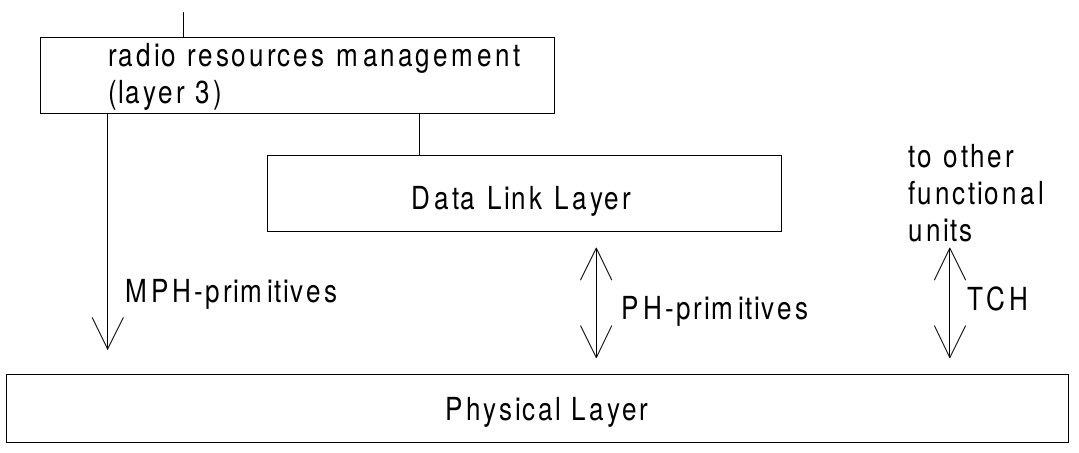
\includegraphics[width=0.7\textwidth]{l1_interfaces}
      \caption{Interfaces with the physical layer~\cite{etsi_gsm_1997}}
      \label{fig:l1_interfaces}
    \end{figure}

  \subsection{Channels}

    This section will first introduce the various logical channels and
    their roles. Then, it will define the physical channels, and
    describe how they are created from multiplexing in the frequency and
    time domains. Finally, it will detail the mapping of the logical
    channels on the physical channels.

    \subsubsection{Logical channels}

      %3GPP TS 44.003 version 12.0.0 Release 12 {
      %and a very little bit of 3GPP TS 45.002 version 12.4.0 Release 12 

      The physical layer offers a transmission service on a limited set
      of logical channels. As already stated, these logical channels are
      of two types: the traffic channels and the control channels.
      Traffic channels are intended to carry encoded speech, while the
      control channels are intended to carry signaling information for
      the layer 3 entities. These two channels can be subdivided in
      subcategories again as shown
      on~\tref{tab:logical_channels}~\cite{3gpp_ts_2014-3,3gpp_ts_2015-4}.

       \begin{table}[h]
          \centering
          \begin{tabular}{@{}lll@{}}
            \toprule
            Type          & Name                    \\
            \midrule

            \multirow{2}{*}{\parbox{0.30\textwidth}{\raggedright Traffic
            Channel (TCH)}} & Full-rate or Bm (TCH/F) \\
                          & Half-rate or Lm (TCH/H) \\

            \\

            \multirow{3}{*}{\parbox{0.30\textwidth}{\raggedright Broadcast
            Channel}} & Frequency Correction Channel (FCCH)\\
                          & Synchronization Channel (SCH)\\
                          & Broadcast Control Channel (BCCH)\\
            \\

            \multirow{3}{*}{\parbox{0.30\textwidth}{\raggedright Common
            Control Channel (CCCH)}} & Random Access Channel (RACH)\\
                          & Access Grant Channel (AGCH)\\
                          & Paging Channel (PCH)\\
            \\
             \multirow{3}{*}{\parbox{0.30\textwidth}{\raggedright
             Dedicated Control Channel (DCCH)}} & Standalone Dedicated Control Channel (SDCCH)\\
                          & Slow Associated Control Channel (SACCH)\\
                          & Fast Associated Control Channel (FACCH)\\
            \bottomrule
          \end{tabular}
          \caption{Logical channels~\cite{3gpp_ts_2015-3}}
          \label{tab:logical_channels}
        \end{table}

      \glspl{tch} can be divided in two categories depending on their
      bit rate capacity: Bm or Full-rate (TCH/F), and Lm or Half-rate
      (TCH/H). Control channels are divided in three subcategories
      depending on their roles: the Broadcast Control channels, the
      \gls{ccch}, and the \gls{dcch}. Each of these can be subdivided
      again.

      The Broadcast Control channels are subdivided into three other
      channels. The \gls{bcch} intended to broadcast a variety of
      information, including information necessary for an \gls{ms} to
      register in the system. The \gls{fcch}, intended for frequency
      correction. And the \gls{sch}, intended for frame synchronization
      and identification of a \gls{bts}.

      The \gls{ccch} is subdivided in three other channels. The
      \gls{rach}, which is the only part of the \gls{ccch} used to
      transmit information from the \gls{ms} to the network. The
      \gls{agch}, which is the part reserved for assignment messages.
      And the \gls{pch}, which is used in the paging process.

      Finally, the \gls{dcch} is subdivided into three channels. The
      \gls{sdcch}, which is a bi-directional \gls{dcch} whose allocation
      is not linked to the allocation of a \gls{tch}. The \gls{facch},
      which is a bi-directional \gls{dcch} obtained by stealing bursts
      from its associated traffic channel. The allocation of a
      \gls{facch} is obviously linked to the allocation of a \gls{tch}.
      And the \gls{sacch}, which is a bi-directional or uni-directional
      \gls{dcch}. An independent \gls{sacch} is always allocated
      together with a \gls{tch} or an \gls{sdcch}.
      %}

    \subsubsection{Physical channels}

      %3GPP TS 45.001 version 12.1.0 Release 12
      %3GPP TS 45.002 version 12.4.0 Release 12 {

      The logical channels mentioned above are mapped on physical
      channels that are described in this section. The complete
      definition of a particular physical channel consists of a
      description in the frequency domain, and a description in the time
      domain~\cite{3gpp_ts_2015-3,3gpp_ts_2015-4}.

      In the frequency domain, the radio spectrum is first divided into
      frequency bands. Each of these bands is then separated between two
      groups, the uplink frequencies, where the mobile transmits and the
      network receives, and the downlink frequencies, where the network
      transmits and the mobile receives. This is the \gls{fdd} scheme.
      Finally, the carrier frequencies are grouped by pair, comprised of
      one carrier frequency in the upper band and one carrier frequency
      in the lower band, to form an \gls{arfcn}. This is the \gls{fdma}
      scheme. Each cell is allocated a subset of these \glspl{arfcn},
      and one of them is used as the beacon channel.

      In the time domain, the access scheme is \gls{tdma} with eight
      basic physical channels per carrier. The basic radio resource is a
      time slot lasting approximately \SI{576.9}{\micro\second}. The
      \gls{gsm} system uses the \gls{gmsk} modulation with a modulation
      rate of around \SI{270.833}{\kilo symbol\per\second}. This means
      that the time slot duration, including guard time, is
      \SI{156.25}{symbols} long. At the \gls{bts} the start of a
      \gls{tdma} frame on the uplink is delayed by the fixed period of 3
      time slots from the start of the \gls{tdma} frame on the downlink.
      This allows the same time slot number to be used in the downlink
      and uplink whilst avoiding the requirement for the \gls{ms} to
      transmit and receive simultaneously. This can be seen
      in~\fref{fig:l1_3ts_hop}.

      \begin{figure}[h]
        \centering
        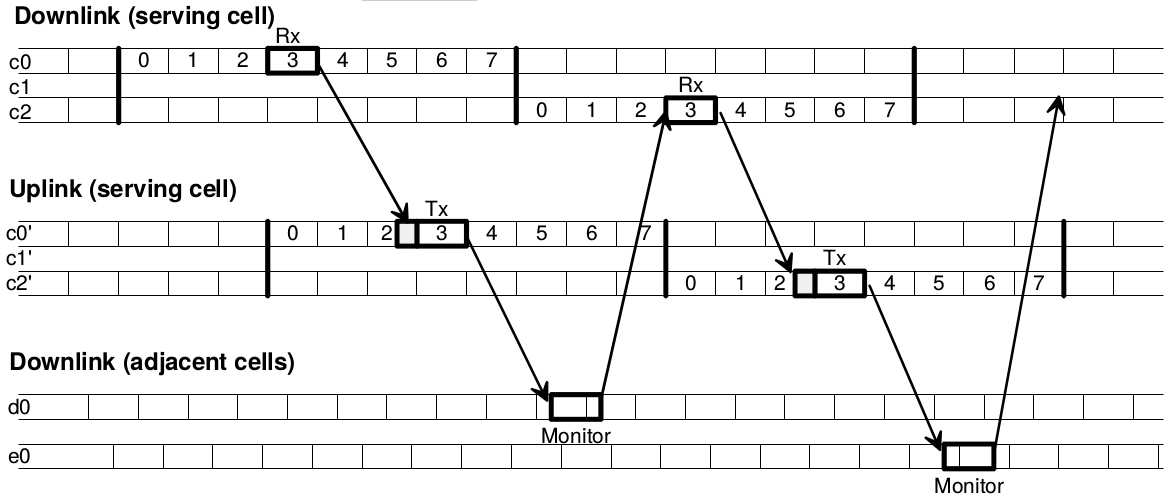
\includegraphics[width=\textwidth]{l1_3ts_hop}
        \caption{Uplink delay and frequency hopping~\cite{3gpp_ts_2015-4}}
        \label{fig:l1_3ts_hop}
      \end{figure}

      The physical content of a time slot is represented by a burst. It
      is defined as a period of a carrier which is modulated by a data
      stream. For the \gls{gmsk} modulation, a symbol represents one bit,
      and thus a burst contains \SI{156.25}{bits}. The period between
      bursts appearing in successive time slots is called the guard
      period and explains the fractional component in the amount of
      bits. Different types of bursts exist in the system, and they are
      displayed on~\fref{fig:bursts}.

      \begin{figure}[h]
        \centering
        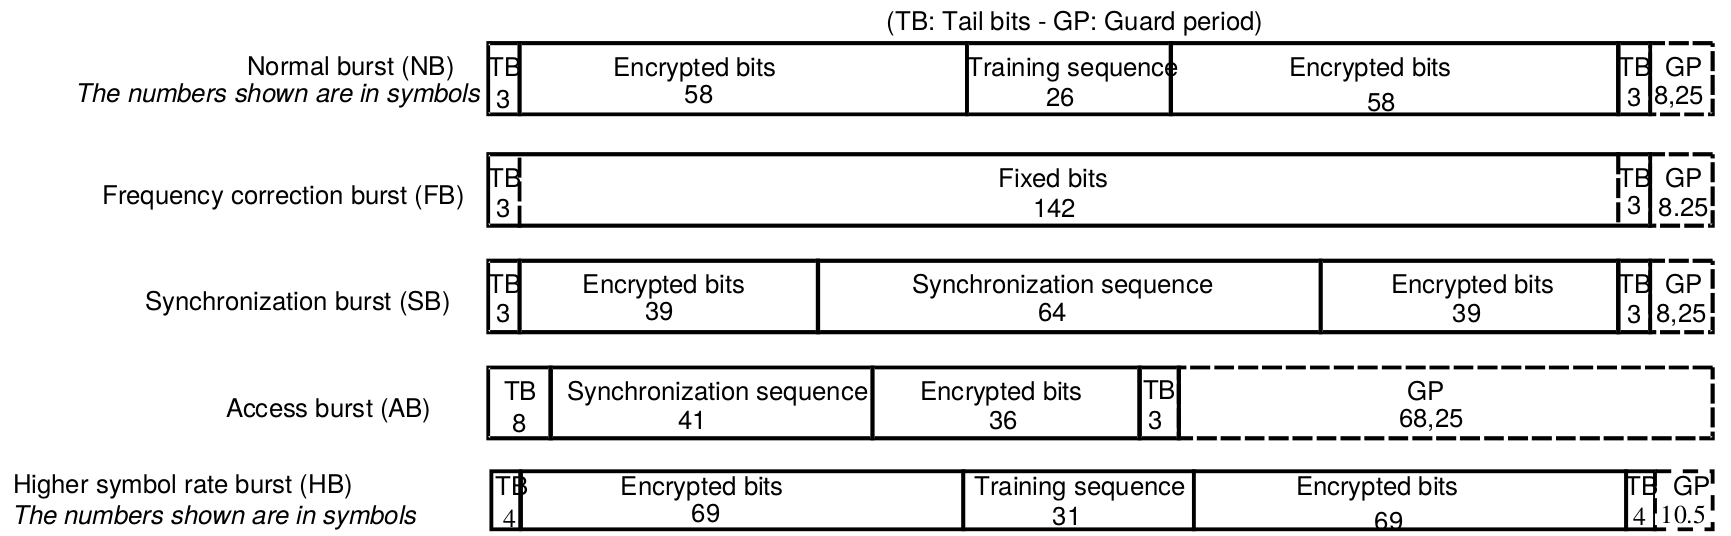
\includegraphics[width=\textwidth]{bursts}
        \caption{Types of bursts~\cite{3gpp_ts_2015-3}}
        \label{fig:bursts}
      \end{figure}

      The frequency hopping capability is optionally used to reduce the
      noise on the communication and is displayed
      on~\fref{fig:l1_3ts_hop}. The principle is that every \gls{ms}
      switches between frequencies according to a given sequence. It
      transmits or receives during one time slot on a fixed frequency
      and must hop on the following before the same time slot on the
      next \gls{tdma} frame. It must be noted that on the beacon
      channel, frequency hopping is not permitted on any time slot
      supporting a \gls{bcch}.
      %}

    \subsubsection{Mapping of the logical channels}

      %3GPP TS 45.001 version 12.1.0 Release 12
      %3GPP TS 45.002 version 12.4.0 Release 12 {

      The \gls{tdma} frames described in the previous section are
      grouped in multiframes. Two types of multiframes exist in the
      system: 26-multiframes comprising 26 \gls{tdma} frames which are
      used to carry traffic channels, and 51-multiframes comprising 51
      \gls{tdma} frames, used to carry signaling channels. These
      multiframes are organized respectively by groups of 51 or 26 to
      form superframes, which are the least common multiple of the time
      frame structures. Finally, 2048 superframes are grouped in
      hyperframes which form the longest recurrent time
      period~\cite{3gpp_ts_2015-3,3gpp_ts_2015-4}.

      \iffalse
      This is shown in~\fref{fig:frames}.
      \begin{figure}[h]
        \centering
        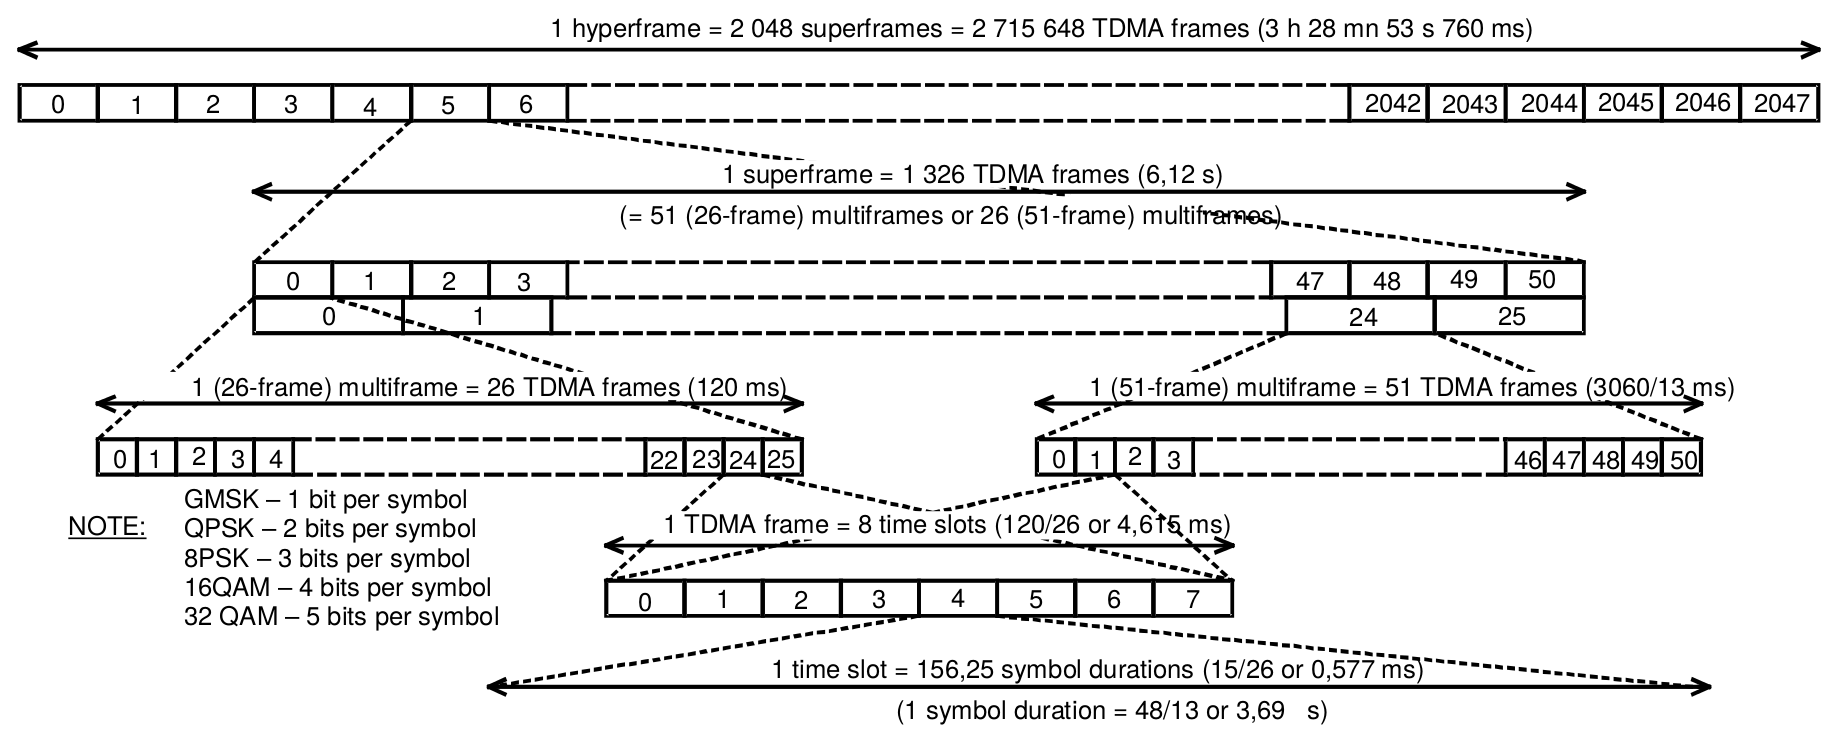
\includegraphics[width=\textwidth]{frames}
        \caption{Logical channels on the 51-multiframe
        ~\cite{3gpp_ts_2015-3}}
        \label{fig:frames}
      \end{figure}
      \fi

      The logical channels are defined by mapping the multiframes on the
      physical channels. For example, on the physical channel composed
      of the time slot $0$ on the beacon frequency, there is a
      $51$-multiframe containing logical channels.
      On~\fref{fig:51multiframe_b-c}, the letter F represents the
      \gls{fcch}, the letter S represents the \gls{sch}, the letter B
      represents the \gls{bcch}, and the letter C represents the
      \gls{ccch}. The \gls{fcch} can be found on time slot $0$ of the
      \gls{tdma} frames $1$, $11$, $21$, $31$, and $41$ of the
      multiframe. This is a kind of \gls{tdma} inside a \gls{tdma}.

      \begin{figure}[h]
        \centering
        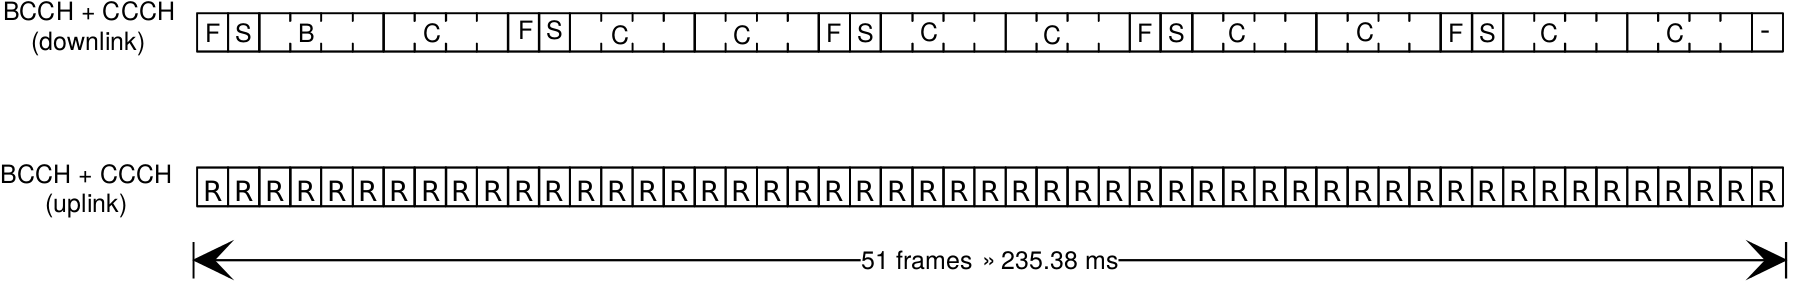
\includegraphics[width=\textwidth]{51multiframe_b-c}
        \caption{3GPP TS 45.001 version 12.1.0 Release 12 20}
        \label{fig:51multiframe_b-c}
      \end{figure}
      %}

  \subsection{Modem}
  \label{sec:modem}
    %3GPP TS 45.001 version 12.1.0 Release 12 {
    %\url{http://bb.osmocom.org/trac/wiki/Rita}
    %~\cite{osmocombb_2015,welte_anatomy_2010}

    The previous section focused on the channels handled by the physical
    layer, and this section will focus on the bitstream transmitted on
    the radio medium. The physical layer is responsible for converting
    the \gls{rf} signals in bursts, and the bursts to packets that can
    be handled by the data link layer. Of course, it is also responsible
    for the inverse operation~\cite{3gpp_ts_2015-3,osmocombb_2015,welte_anatomy_2010}.

    The physical layer is highly dependent on the hardware, and it is
    therefore interesting to take a look at the platform supported by
    the \proj{OsmocomBB} project. This platform is the \gls{ti} Calypso
    based modem from which a block schematic is represented
    on~\fref{fig:calypso_modem}. The Calypso based modem includes an
    \gls{rf} frontend, an \gls{abb}, and a \gls{dbb}.

    \begin{figure}[h]
      \centering
      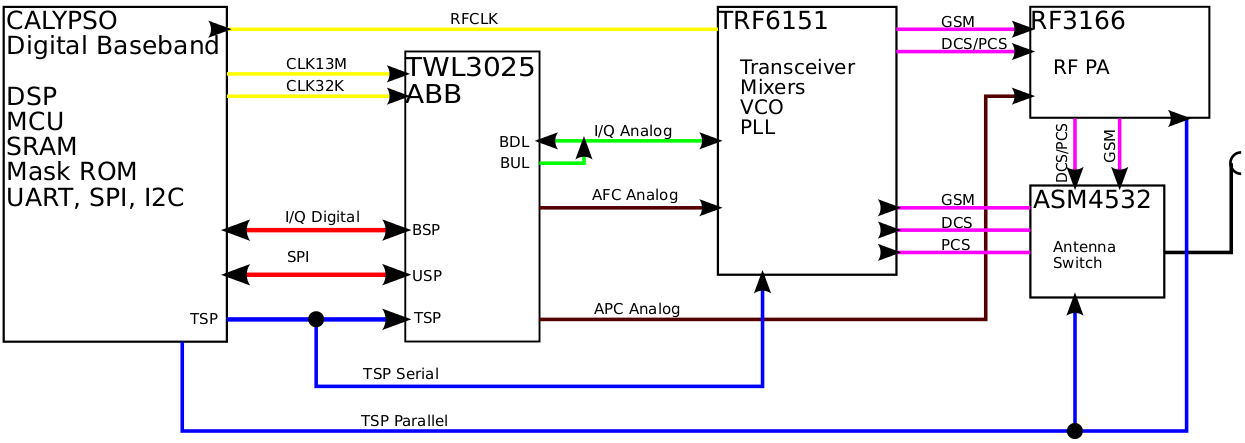
\includegraphics[width=\textwidth]{calypso-block}
      \caption{Block diagram of a typical Calypso based
              modem~\cite{welte_anatomy_2010}}
      \label{fig:calypso_modem}
    \end{figure}

    The \gls{rf} frontend is used to receive and transmit at the GSM
    frequency, and is composed of an antenna switch, an \gls{rf} power
    amplifier controlling the output level, and a \gls{ti} Rita GSM
    transceiver. The antenna switch routes the signal to the receive or
    transmit path. On the receive path, the signal is filtered and
    amplified to prevent noise. Then, it is mixed with a frequency
    generated by the local oscillator and filtered again to convert it
    from the \gls{gsm} frequency to a baseband signal. Finally, this
    baseband signal is sent to the \gls{abb}. On the transmit path, the
    \gls{rf} frontend receives a signal from the \gls{abb}, converts it
    to the relevant \gls{gsm} frequency, sends it to the \gls{rf} power
    amplifier shown on the top right of the schematic, and sends it to
    the antenna switch which now connects the transmit path with the
    antenna.

    The \gls{ti} Iota \gls{abb} deals with the sampling, the
    differential encoding, and the modulation. On the receive path, when
    the \gls{abb} receives the analog signal from the \gls{rf} frontend,
    it simply filters and samples it in an \gls{adc}, before sending the
    digital samples to the \gls{dbb}. On the transmit path, the
    \gls{abb} receives digital signals from the \gls{dsp}, modulates
    them and converts them to analog signals in a \gls{dac}. The
    modulation is done in the \gls{abb} because it is much simpler to
    apply a \gls{gmsk} modulation than a demodulation. This reduces the
    complexity of the \gls{dsp}, and therefore its cost and power
    consumption.

    The \gls{ti} Calypso \gls{dbb} on the left is composed of a
    \gls{dsp} and an \comp{ARM7TDMI} processor. The \gls{dsp} is
    responsible for the the demodulation, the burst building and
    multiplexing, the encryption, the interleaving, reordering and
    partitioning, and finally the coding. The \comp{ARM7} processor is
    called the Baseband Processor and runs the \proj{OsmocomBB}
    implementation of the \gls{gsm} \gls{ms} protocol stack.

    \proj{OsmocomBB} implements the drivers for the various components
    of the platform: the \gls{rf} transceiver, the \gls{abb}, or the
    \gls{dsp}, but also the keypad, the display, and so on. For example,
    the \gls{dsp} communicates with the baseband processor using an API
    available through a shared memory interface. \proj{OsmocomBB} does
    not modify the code inside the \gls{dsp}, but drives it by
    implementing this API. Therefore, code running on the baseband
    processor can use the various tasks provided by the \gls{dsp}.

  \subsection{Procedures}
  %3GPP TS 44.004 version 12.0.0 Release 12{
    %3GPP TS 44.005 version 12.0.0 Release 12 5 {

    To provide its various services, the physical layer implements three
    types of procedures. The first ones are the control procedures,
    which handle the control of the various channels. These procedures
    are composed of primitives between the physical layer and the
    \gls{rr} sublayer of the layer 3. The second ones are the interface
    procedures. They are composed of four kind of primitives between the
    physical layer and the data link layer. The first kind is used for
    connection establishment, the second one is used for data
    transmission, the third is used for random access over the
    \gls{rach}, and the last one is used for transmission and
    synchronization. A third type of procedure exists to handle the
    traffic channels~\cite{3gpp_ts_2014-4,3gpp_ts_2014-5,osmocombb_ms-side_????}.
    %}

    All these primitives are implemented in the \proj{OsmocomBB}
    \prog{layer 1} application running on the baseband processor. They
    make use of the hardware detailed in the previous section by using
    the various drivers and the \gls{dsp} API. This application also
    implements the various schedulers needed to use these primitives at
    the right time.

    The layer 1 can be divided in two main parts: the synchronous and
    the asynchronous part. The first one is executed synchronously with
    the \gls{tdma} frame clock thanks to interrupts at every new
    \gls{tdma} frame. The second one uses the data provided by the
    synchronous part and schedules the next actions. It also typically
    communicates with the upper layers, which run on a computer and
    communicate with the layer 1 using the L1CTL interface through a
    serial connection. This interface is implemented in
    \code{src/target/firmware/layer1/l23\_api.c} on the \gls{ms} side,
    and in \code{src/host/layer23/src/common/l1ctl.c} on the computer
    side.

\section{Data link layer}

%3GPP TS 44.005 version 12.0.0 Release 12 5 {
  The data link layer is the second layer of the \gls{gsm} \gls{ms}
  protocol stack. It uses the signaling channels established by the
  physical layer to provide data link connections to the layer 3 by
  implementing a protocol called \gls{lapdm}, where Dm channel is
  another name to designate the signaling channels. This protocol can
  initiate acknowledged or unacknowledged data link connections. The
  first ones implement error recovery procedures and flow control, while
  the second ones do not~\cite{3gpp_ts_2014-5}.   
%}

  \subsection{Procedures}

%3GPP TS 44.005 version 12.0.0 Release 12 5 {
  The data link layer provides two relevant procedures: the random
  access procedure, and the data link procedure. The random access
  procedure is used for data links on the \gls{rach} to format and
  initiate the transmission of the random access frames~\cite{3gpp_ts_2014-5}.

  The data link procedure is used to transmit information between layer
  3 entities across the Um interface. It can handle to types of
  operations: acknowledged and unacknowledged. The first one implements
  error recovery procedures and flow control, and handles numbered
  information frames that are acknowledged by the receiving data link
  layer. It also offers segmentation of layer 3 messages if they do not
  fit in one frame. The second one does not implement any of this and
  handles unnumbered information frames. The \gls{bcch}, the \gls{pch},
  and the \gls{agch} will only support unacknowledged operation, and the
  \gls{dcch} will support both types.
%}

  %http://events.ccc.de/congress/2010/Fahrplan/attachments/1771_osmocombb-27c3.pdf
  %{
  These procedures are performed using three types of primitives. The
  first one is associated with random access, the second one is
  associated with the unacknowledged information transfer service, and
  the last one is associated with the multiple frame acknowledged
  information transfer services. All these primitives are implemented in
  \proj{OsmocomBB} in the \code{src/shared/libosmocore/gsm/lapdm.c} and
  \code{src/shared/libosmocore/gsm/lapd\_core.c} files. Since the data
  link layers are similar on both side of the Um interface, the code
  used in the \proj{OpenBSC} project is reused and extended when
  necessary, and this is why it can be found in the
  \code{src/shared/libosmocore/} directory. The data link layer
  communicates with the physical layer over a serial communication using
  the L1CTL interface. It also communicates with the layer 3 using the
  RSLms interface~\cite{osmocombb_ms-side_????,welte_osmocombb:_2010-1}.
  %}

  \iffalse
  %http://events.ccc.de/congress/2010/Fahrplan/attachments/1771_osmocombb-27c3.pdf {
  interface between Layer2 and Layer3 called RSLms
  In the GSM network, Um Layer2 terminates at the BTS but
  is controlled by the BSC
  Reuse this GSM 08.58 Radio Signalling Link
  Extend it where needed for the MS case
  %}
  \fi

\section{Layer 3}

%3GPP TS 24.007 version 12.0.0 Release 12 22 {
  The last layer of the \gls{gsm} \gls{ms} protocol stack is the layer
  3. It is composed of three sublayers: the \gls{rr} sublayer, the
  \gls{mm} sublayer, and the \gls{cm} sublayer. The \gls{cm} sublayer is
  further divided into functional blocks including the mandatory blocks
  for \gls{ss}, \gls{sms}, and \gls{cc}~\cite{3gpp_ts_2014-6}.

  %} 3GPP TS 44.018 version 12.5.0 Release 12{
  Complete layer 3 transactions consist of specific sequences of
  elementary procedures. Therefore, the following sections will describe
  these procedures for each of the sublayers. The last section will then
  provide an example for a complete \gls{mtc}, which involves all the
  procedures described here.
  
  Since all these procedures are implemented in the \prog{mobile}
  application of \proj{OsmocomBB}, output of this application is
  provided as practical examples. Each line of the logs contains the
  file name, followed by the line number, and the message. For example:
  \code{gsm48\_rr.c:4820 Channel provides data}. This is an easy way to
  find were a given procedure is implemented.The code of this
  application can be found in the \code{src/host/layer23/src/mobile/}
  directory~\cite{3gpp_ts_2015-2,osmocombb_ms-side_????}.
    %}

  \iffalse
  The procedures introduced in this section are placed in context in
  complete examples in \Sref{} and \Sref{}. They are also shown in
  \Sref{}, where the use of the \proj{OsmocomBB} applications is
  demonstrated. 
  \fi

  \subsection{Radio Resource Management procedures}
  \label{sec:rr_proc}

    %3GPP TS 44.018 version 12.5.0 Release 12{
    \gls{rr} procedures include the functions related to the management
    of the control channels and the data link connections on these
    channels. They are implemented in the \prog{mobile} application of
    \proj{OsmocomBB} in the \code{mobile/gsm48\_rr.c} and
    \code{mobile/gsm322.c} file. Their general purpose is to establish,
    maintain and release \gls{rr} connections that allow a dialogue
    between the network and a mobile station. When a connection is
    established, the \gls{rr} sublayer is in dedicated mode. When a
    connection is not established, it is in idle
    mode~\cite{3gpp_ts_2015-2}.

    When in idle mode, the \gls{rr} procedures include the reception and
    measurement of the \gls{bcch} and \gls{ccch}. The measurements are
    coming from the physical layer and are treated to assess the need of
    a cell change. The way it happens in the \prog{mobile} application
    is shown through logs displayed on \fref{fig:pm}, \fref{fig:pm2},
    and \fref{fig:pm3}. The \gls{ms} will first measure the power level
    of all the neighboring cells, then try to synchronize to each of
    them and read their system information messages, and finally deduce
    the cell reselection parameters. These parameters are used to
    determine if a cell change is needed~\cite{3gpp_ts_2014-8}.

      \begin{figure}[p]
        \centering
        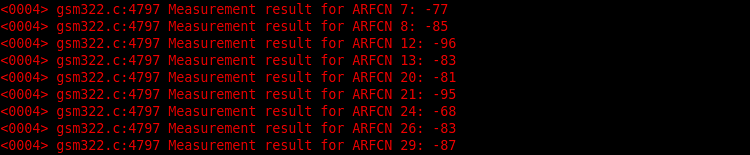
\includegraphics[width=\textwidth]{pm}
        \caption{Power measurements logs in \prog{mobile}: signal
        strength}
        \label{fig:pm}
      \end{figure}

      \begin{figure}[p]
        \centering
        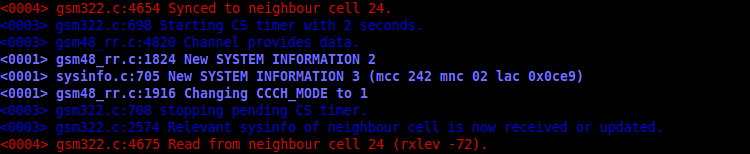
\includegraphics[width=\textwidth]{pm2}
        \caption{Power measurements logs in \prog{mobile}: System
        Information messages}
        \label{fig:pm2}
      \end{figure}

      \begin{figure}[p]
        \centering
        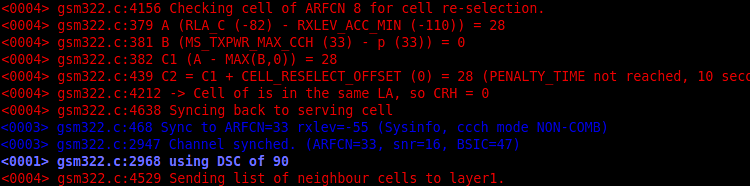
\includegraphics[width=\textwidth]{pm3}
        \caption{Power measurements logs in \prog{mobile}: reselection
        parameters}
        \label{fig:pm3}
      \end{figure}

    To switch from idle mode to dedicated mode, an immediate assignment
    procedure can be initiated by the \gls{rr} sublayer of the \gls{ms}
    in two cases. Firstly, upon reception of a request from the \gls{mm}
    sublayer to enter the dedicated mode. Secondly, in response to a
    Paging Request message assigned to its \gls{tmsi} or \gls{imsi}, and
    received when listening to the \gls{ccch}. In these cases, the
    \gls{rr} sublayer schedules the sending on the \gls{rach} of a
    Channel Request message containing an establishment cause and a
    random reference. Then, it waits until reception of an Immediate
    Assignment message, which contains information regarding the
    \gls{dcch} assigned to the \gls{ms}. If it receives an Immediate
    Assignment Reject or if it does not receive any message after the
    maximum amount of Channel Request messages have been sent, the
    \gls{rr} sublayer aborts the procedure. A successful immediate
    assignment procedure in the \prog{mobile} application is shown on
    \fref{fig:mobile_rach}.

      \begin{figure}[p]
        \centering
        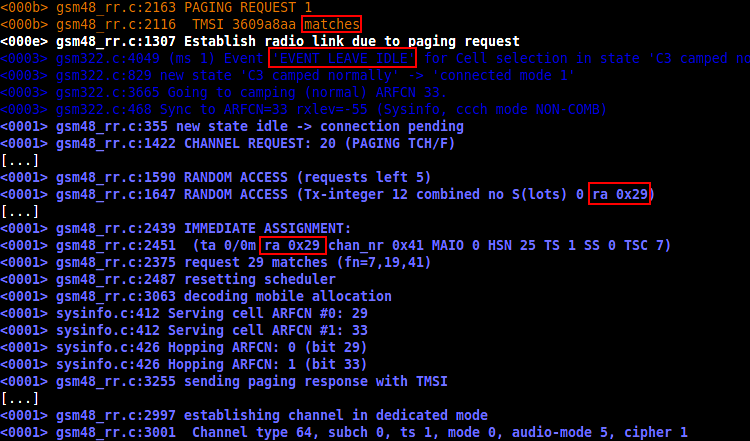
\includegraphics[width=\textwidth]{mobile_rach}
        \caption{Immediate assignment procedure logs in \prog{mobile}}
        \label{fig:mobile_rach}
      \end{figure}

    When in dedicated mode, the network can initiate the dedicated
    channel assignment procedure by sending an Assignment Command
    message to the \gls{ms} on the main signaling link. Upon reception,
    the \gls{ms} commands to switch to the assigned channels described
    in the message. If the main signaling link is successfully
    established, the \gls{ms} returns an Assignment Complete message to
    the network on the main \gls{dcch}. If the establishment fails, it
    sends an Assignment failure instead. A successful procedure in the
    \prog{mobile} application is shown on \fref{fig:mobile_asscmd}.

      \begin{figure}[p]
        \centering
        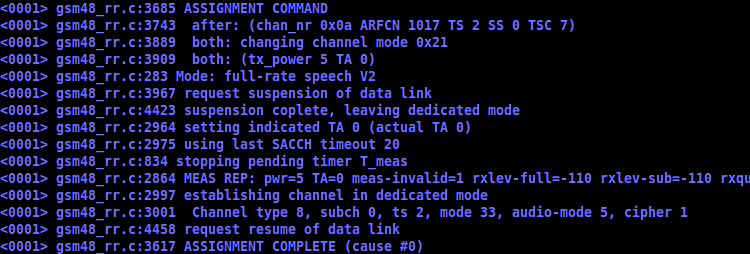
\includegraphics[width=\textwidth]{mobile_asscmd}
        \caption{Dedicated channel assignment procedure logs in \prog{mobile}}
        \label{fig:mobile_asscmd}
      \end{figure}

    In dedicated mode, the network can also initiate a ciphering mode
    setting procedure by sending a Ciphering Mode Command message. This
    contains information about the encryption algorithm to use, if any.
    The \gls{ms} answers with a Ciphering Mode complete message when the
    procedure is over. An example in the \prog{mobile} application is
    given in \fref{fig:mobile_mm}. To go back to idle mode, the
    connection release procedure can be triggered by upper layers, which
    deactivates all the dedicated channel in use. This can be used after
    a call, or when a dedicated channel assigned for signaling is
    released.
    %}

  \subsection{Mobility Management procedures}

    %3GPP TS 24.008 version 12.9.0 Release 12 {
    The \gls{mm} sublayer is used to support the mobility of the various
    \glspl{ms}. For example, by informing the network of their
    locations, or by providing user identity confidentiality. It also
    provides connection management services to the various entities of
    the \gls{cm} sublayer, as well as registration services to the upper
    layers directly. To perform these services, it relies on the
    \gls{rr} sublayer to establish a connection between the \gls{ms} and
    the network~\cite{3gpp_ts_2015-5}. 
    %}

    %3GPP TS 24.008 version 12.9.0 Release 12 {
    Depending on how they are initiated, three types of \gls{mm}
    procedures can be distinguished: common procedures, specific
    procedures, and connection management procedures. All of these will
    be investigated in turn. This section does not provide an exhaustive
    list of procedures, but focuses on the relevant ones for this
    thesis. All these procedures are implemented in the \prog{mobile}
    application again. The code can be found in the
    \code{src/host/layer23/src/mobile/gsm48\_mm.c} file.

    \subsubsection{Common procedures}
    \label{sec:mm_proc_com}

    The purpose of the \gls{tmsi} reallocation procedure is to prevent a
    user from being identified and located by an attacker. Usually it is
    performed at least at each location area change. The network
    initiates this procedure by sending a \gls{tmsi} Reallocation
    Command message to the \gls{ms} containing a new combination of
    \gls{tmsi} and \gls{lai}.  Upon reception, the \gls{ms} stores them
    in the SIM and sends a \gls{tmsi} Reallocation Complete message to
    the network.

    The purpose of the authentication procedure is twofold: it permits
    the network to check whether the identity provided by the \gls{ms}
    is acceptable or not, and it provides parameters enabling the
    \gls{ms} to calculate a new ciphering key. This procedure is always
    controlled by the network which initiates it by sending an
    Authentication Request message. The \gls{ms} then processes the
    challenge information, computes a new key, and sends back an
    Authentication Response message to the network. If it is not valid,
    the network sends an Authentication Reject message to the \gls{ms}.

      \begin{figure}[p]
        \centering
        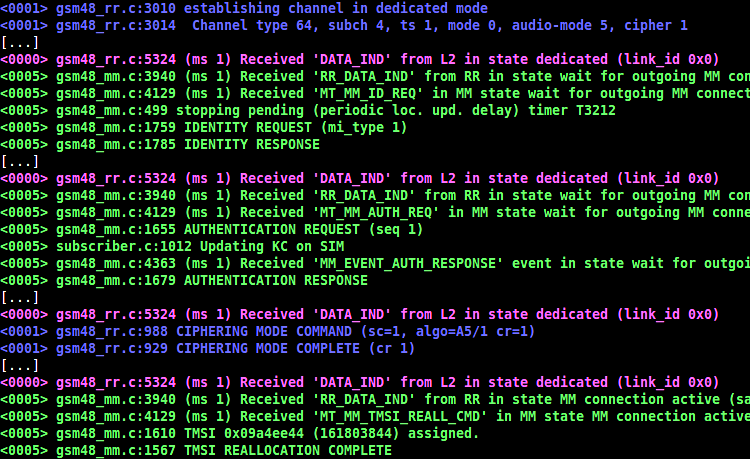
\includegraphics[width=\textwidth]{mobile_mm}
        \caption{Identification, authentication, ciphering mode setting, and TMSI
        reallocation procedures logs in \prog{mobile}}
        \label{fig:mobile_mm}
      \end{figure}

    The identification procedure is used by the network to request an
    \gls{ms} to provide specific identification parameters to the
    network, like its \gls{imsi} or \gls{imei}. The network initiates
    the identification procedure by transferring an Identity Request
    message. Upon reception, the \gls{ms} sends back an Identity
    Response message containing the identification parameters as
    requested by the network. An example of these three procedures in
    the \prog{mobile} application is shown on \fref{fig:mobile_mm}.

    The \gls{imsi} detach procedure may be invoked by an \gls{ms} if the
    phone is turned off or if the \gls{sim} is removed. It consists of
    the \gls{imsi} Detach Indication message sent from the \gls{ms} to
    the network. When receiving this message, the network may set an
    inactive indication for the \gls{imsi}, but this is optional. No
    response is returned to the mobile station. This procedure is shown
    in the \prog{mobile} application on \fref{fig:mobile_detach}.

      \begin{figure}[p]
        \centering
        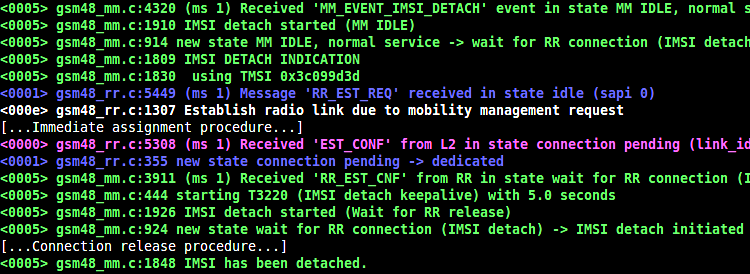
\includegraphics[width=\textwidth]{mobile_detach_s}
        \caption{IMSI detach procedure logs in \prog{mobile}}
        \label{fig:mobile_detach}
      \end{figure}

    \subsubsection{Specific procedures}
    \label{sec:mm_proc_spec}

    The specific procedures are all variations of the location updating
    procedure, which is used for the following purposes: normal location
    updating, periodic updating, or \gls{imsi} attach. All of them
    follow the same pattern and are initiated by the \gls{ms} which
    sends a Location Updating Request message specifying the location
    update variation to the network. The network might then initiate
    various common procedures, for example a \gls{tmsi} reallocation or
    an identification procedure to obtain needed parameters. Depending
    on these parameters, it answers with a Location Updating Accept or
    Reject message.

    The normal location updating procedure is used to update the
    registration of the current location area of an \gls{ms} in the
  network. The \gls{ms} will also start the normal location updating
  procedure if the network indicates that the mobile station is
  unknown in the \gls{vlr} as a response to an \gls{mm} connection
  establishment request. Periodic updating may be used to notify the
  availability of the \gls{ms} to the network at specified intervals.
  The \gls{imsi} attach procedure is the complement of the \gls{imsi}
  detach procedure, and is used to indicate the \gls{imsi} as active
  in the network. An example of an \gls{imsi} attach procedure in
  \prog{mobile} is shown on \fref{fig:mobile_loc_up} and
  \fref{fig:mobile_loc_acc}.

    \begin{figure}[p]
      \centering
      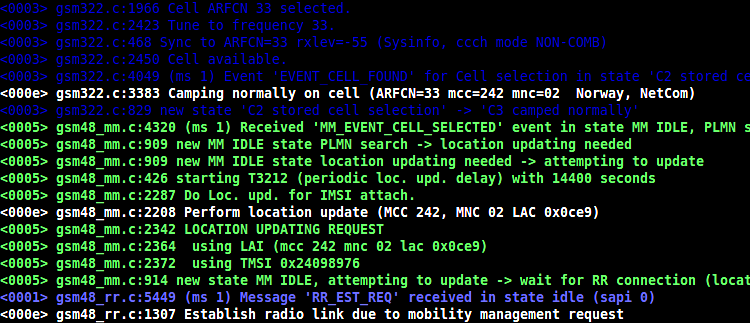
\includegraphics[width=\textwidth]{mobile_loc_up}
      \caption{IMSI attach procedure logs in \prog{mobile}: Location
      Updating Request}
      \label{fig:mobile_loc_up}
    \end{figure}

    \begin{figure}[p]
      \centering
      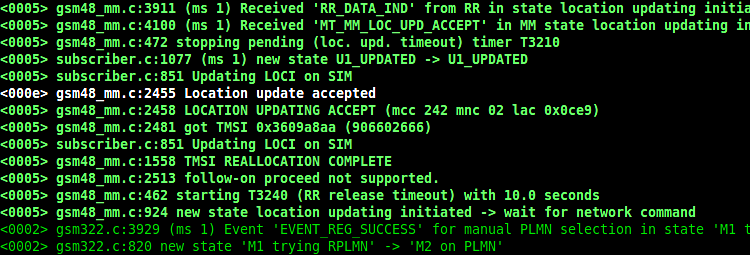
\includegraphics[width=\textwidth]{mobile_loc_acc}
      \caption{IMSI attach procedure logs in \prog{mobile}: Location
      Updating Accept}
      \label{fig:mobile_loc_acc}
    \end{figure}

  \subsubsection{Connection management procedures}

  The \gls{mm} sublayer provides connection management services to the
  various entities of the upper \gls{cm} sublayer upon request from a
  \gls{cm} entity. The connection management procedures are used for
  establishing, re-establishing, maintaining, and releasing an
  \gls{mm} connection.

  In order to establish an \gls{mm} connection, the \gls{mm} sublayer
  sends a \gls{cm} Service Request message to the network. Upon
  reception, the network may start any of the \gls{mm} common
  procedures and \gls{rr} procedures to obtain further information on
  the \gls{ms}. Upon reception of a \gls{cm} Service Accept message,
  the \gls{cm} entity that requested the \gls{mm} connection is
  informed, and the connection is considered to be active. If the
  service request can not be accepted, the network returns a \gls{cm}
  Service Reject message to the \gls{ms}.

  After the \gls{mm} connection has been established, it can be used
  by the \gls{cm} sublayer entity for information transfer. A \gls{cm}
  sublayer entity can then request the transfer of \gls{cm} messages
  which are sent to the \gls{mm} sublayer and transfered to the other
  side of the Um interface. Upon receiving a \gls{cm} message, the
  \gls{cm} sublayer will distribute it to the relevant \gls{cm}
  entity. If the received message is the first for the \gls{mm}
  connection, the \gls{mm} sublayer will in addition indicate to that
  entity that a new connection has been established. An established
  \gls{mm} connection can be released by the local \gls{cm} entity.
  This is done locally in the \gls{mm} sublayer without sending
  messages over the radio interface for this purpose.

  \subsubsection{Location updating example}

  An example of the Location updating procedure is shown on
  \fref{fig:flow_loc_upd}. The \gls{mm} sublayer of the \gls{ms}
  requests an \gls{rr} connection establishment. The \gls{rr} sublayer
  then starts the immediate assignment procedure and sends a Channel
  Request messages on the \gls{rach}. The network answers with an
  Immediate Assignment message.

  Once the dedicated channel is established, the \gls{mm} sublayer
  performs the authentication procedure. Then the ciphering mode
  setting procedure is completed between the \gls{rr} sublayer
  entities. An identification procedure and a \gls{tmsi}
  reallocation procedure could also be scheduled at this point.
  Finally, the network \gls{mm} sublayer sends a Location Updating
  Accept message, and the connection is released.

    \begin{figure}[h]
      \centering
      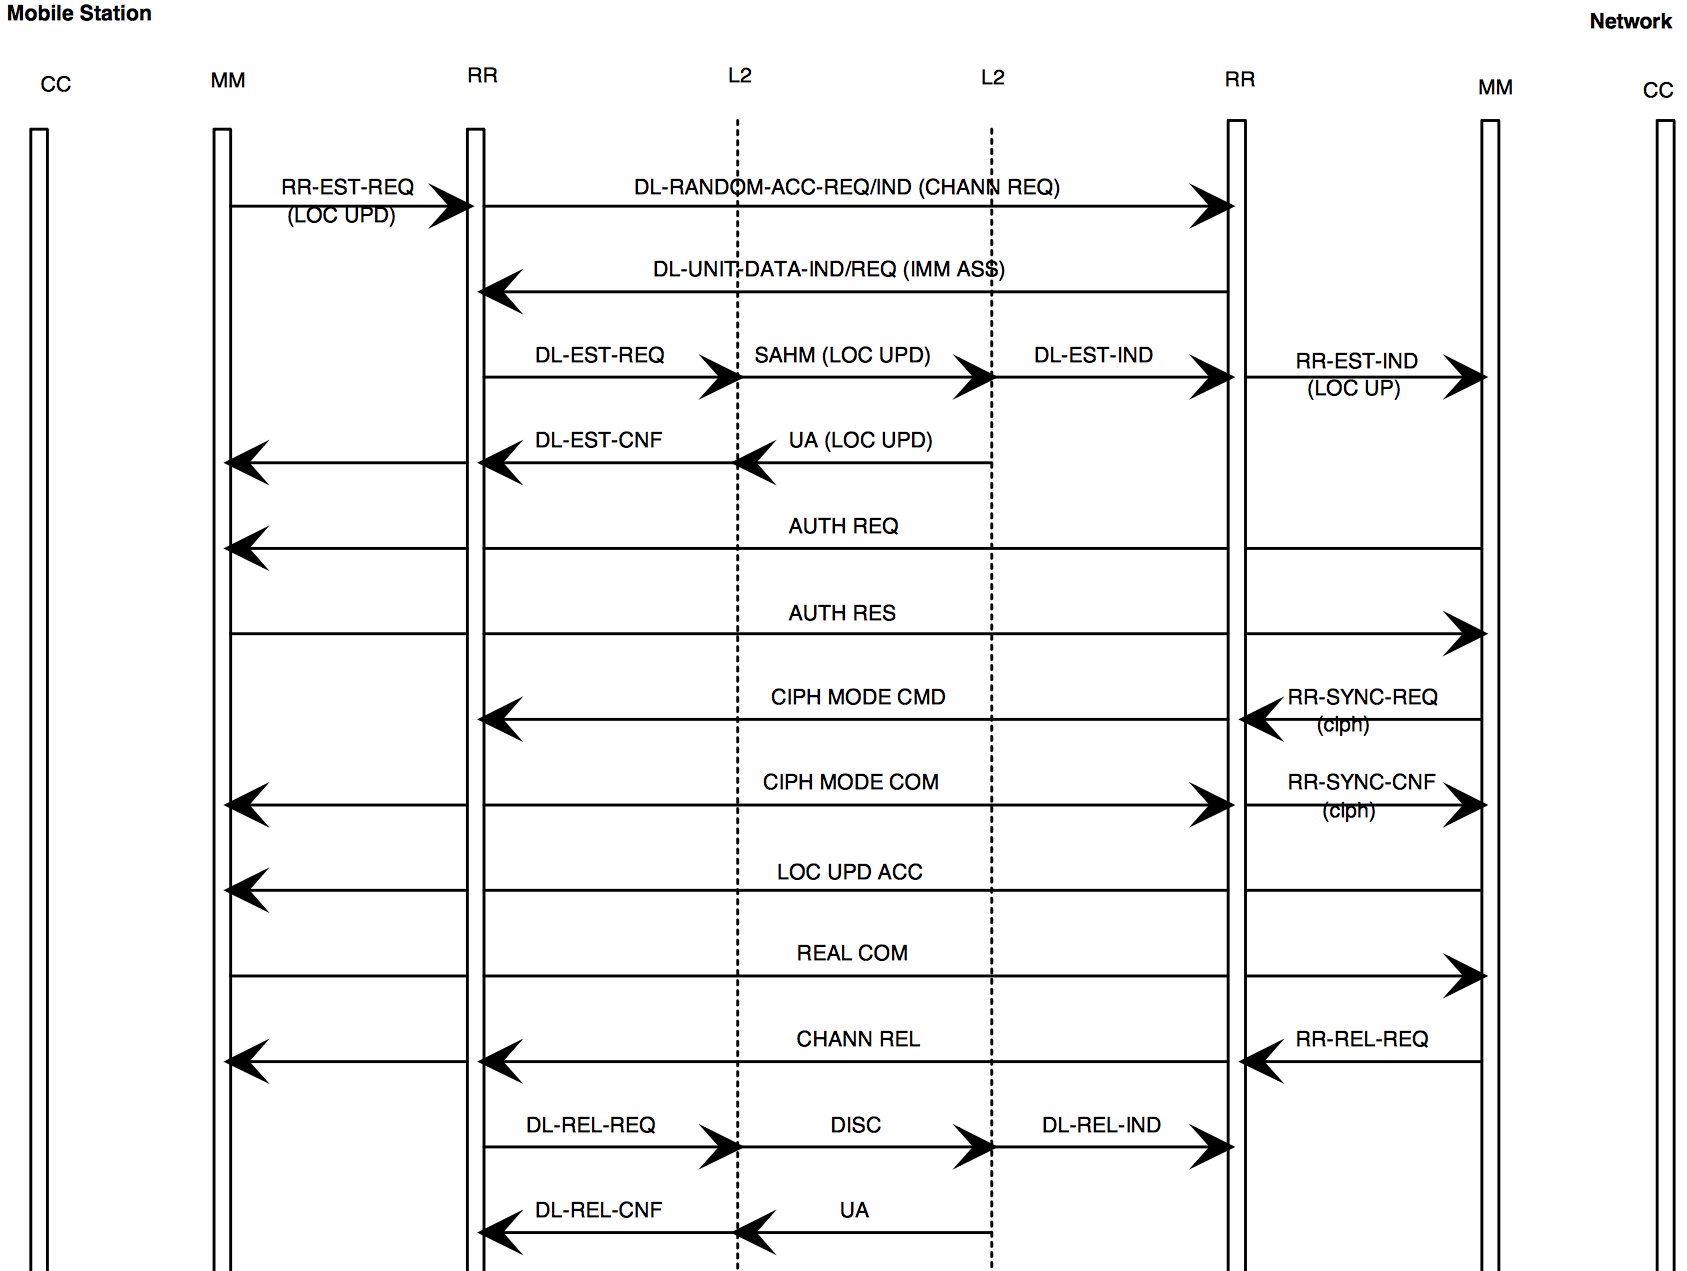
\includegraphics[width=\textwidth]{flow_loc_upd}
      \caption{Location updating procedure flow
      diagram~\cite[p.~117]{3gpp_ts_2014-6}}
      \label{fig:flow_loc_upd}
    \end{figure}

\subsection{Connection Management}

  %3GPP TS 24.008 version 12.9.0 Release 12 {
  The \gls{cm} sublayer relies on the \gls{mm} sublayer to provide
  connection management services. It is subdivided in at least three
  mandatory entities: the \gls{ss} entities, the \gls{sms} entities,
  and the \gls{cc} entities. The last one is used for establishing,
  maintaining, and releasing normal voice calls, whether they are
  \gls{moc} or \gls{mtc}, or \gls{moc} emergency calls. It is
  implemented in the \code{mobile/gsm48\_cc.c} file. The other
  entities are not investigated here~\cite{3gpp_ts_2015-5}.
%}
  \iffalse
  \subsubsection{Short Message Services}

    %3GPP TS 24.011 version 12.0.0 Release 12 {o
  The \gls{sms} entity on the \gls{ms} implements two protocols to
  communicate over the Um interface: the \gls{smcp}, and the
  \gls{smrp}. The first one is used to communicate between two
  \gls{smc} entities, while the second one is used to communicate
  between two \gls{smr} entities. An \gls{smc} entity is part of the
  \gls{cm} sublayer and provides services to the \gls{smr} entity,
  part of the \gls{smr} layer. Finally, the \gls{smr} layer provides
  services to the \gls{smt} layer. 

  When a message transfer is requested by the \gls{smt} layer, the
  \gls{smr} entity sends an RP-Data message to the \gls{smc} entity.
  The \gls{smc} entity will then establish an \gls{mm} connection and,
  when it is ready, send a CP-Data message. If the receiving \gls{smc}
  entity can accept the data, it transmits the message to the
  \gls{smr} layer and answers with a CP-Ack message. Otherwise it
  sends a CP-Error message. The sending \gls{smc} entity will then
  respectively transmit an RP-Ack or RP-Error message to the sending
  \gls{smr} entity.

  These procedures are implemented in the \prog{mobile} application of
  \proj{OsmocomBB} and can be found in
  \code{mobile/gsm411\_sms.c}.
    %}
  \fi

  \subsubsection{Call Control procedures}

%3GPP TS 24.008 version 12.9.0 Release 12 {
  Two \gls{cc} entity procedures are relevant: the call establishment
  procedures, and the call clearing procedures. The call establishment
  procedures consists of several steps and can be of two types: the
  \gls{moc} establishment, or the \gls{mtc} establishment. Both of
  them are reviewed together. An example of the whole procedure is
  described in the next section.

  On the originating \gls{ms}, the \gls{cc} entity initiates
  establishment of a \gls{cc} connection by requesting the \gls{mm}
  sublayer to establish an \gls{mm} connection. Upon establishment of
  this connection, the \gls{cc} entity sends a Setup or Emergency
  Setup message to the network. The setup message will contain all
    the information required by the network to process the call. The
    network answers with a Call Proceeding message to indicate that the
    call is being processed.

    The network will then indicate the arrival of a call to the
    terminating \gls{ms} which will establish a \gls{cc} connection to
    receive the Setup message. Upon reception, it will answer with a
    Call confirm message. It will then start alerting the user and send
    an Alerting message to the network. The network transfers the
    Alerting message to the originating \gls{ms}. If the terminating
    \gls{ms} accepts the call, it sends a Connect message to the
    network. The network will answer with a Connect Acknowledge message,
    connect the traffic channel between the two parties, and send  a
    Connect message to the originating \gls{ms}. The later answers with
    a Connect Acknowledge message and will attach the user connection.

    The clearing procedure is started when either of the two parties
    sends a Disconnect message to the network. Upon reception, the
    network sends a Release message to the other party and starts the
    procedures to release the connections. The \gls{ms} answers with a
    Release Complete message.

    \subsection{Mobile Terminating Call example}

    This section gives an example of a successful \gls{mtc}
    establishment and release. Flow diagrams are available in
    \fref{fig:flow_mtc_setup} and \fref{fig:flow_moc_release}, and logs
    of the \prog{mobile} applications are show in
    \fref{fig:mobile_mtc_setup} and \fref{fig:mobile_mtc_release}. These
    two examples use most of the procedures described in this chapter,
    and will serve as a summary.

    On the flow diagram of \fref{fig:flow_mtc_setup}, the procedure is
    initiated by the \gls{cc} entity of the network, which requests the
    establishment of an \gls{mm} connection. The \gls{mm} sublayer then
    requests an \gls{rr} connection, and the \gls{rr} sublayer starts
    the immediate assignment procedure. It consists of the Paging
    Request, Channel Request, and Immediate Assignment messages. When it
    is over, the \gls{mm} sublayer in the network receives an \gls{rr}
    Establishment Confirmation, while the \gls{mm} sublayer in the
    \gls{ms} receives an \gls{rr} Establishment Indication.

    When the channel is established, the authentication procedure
    between the \gls{mm} sublayers starts. This can be followed by the
    identification procedure, which is not displayed on this diagram.
    Then the \gls{rr} sublayer of the network initiates a ciphering mode
    setting procedure. Again, this could be followed by a \gls{tmsi}
    reallocation procedure which is not shown.
    
    At this point, the \gls{cc} entity on the network side receives an
    \gls{mm} Establishment Confirmation, and sends the Setup message to
    the \gls{cc} entity on the \gls{ms}. This message is also used as an
    \gls{mm} Establishment Indication message. If the establishment
    succeeds, the communication will switch to a traffic channel thanks
    to the dedicated channel assignment procedure. When on the traffic
    channel, the call setup is resumed, and if it succeeds, the voice
    data starts flowing.

    The clearing procedure is displayed on \fref{fig:flow_moc_release}.
    The \gls{cc} entities release the \gls{mm} connection. The \gls{mm}
    sublayer releases the \gls{rr} connection, and finally the data link
    layer releases the data link connection.

      \begin{figure}[h]
        \centering
        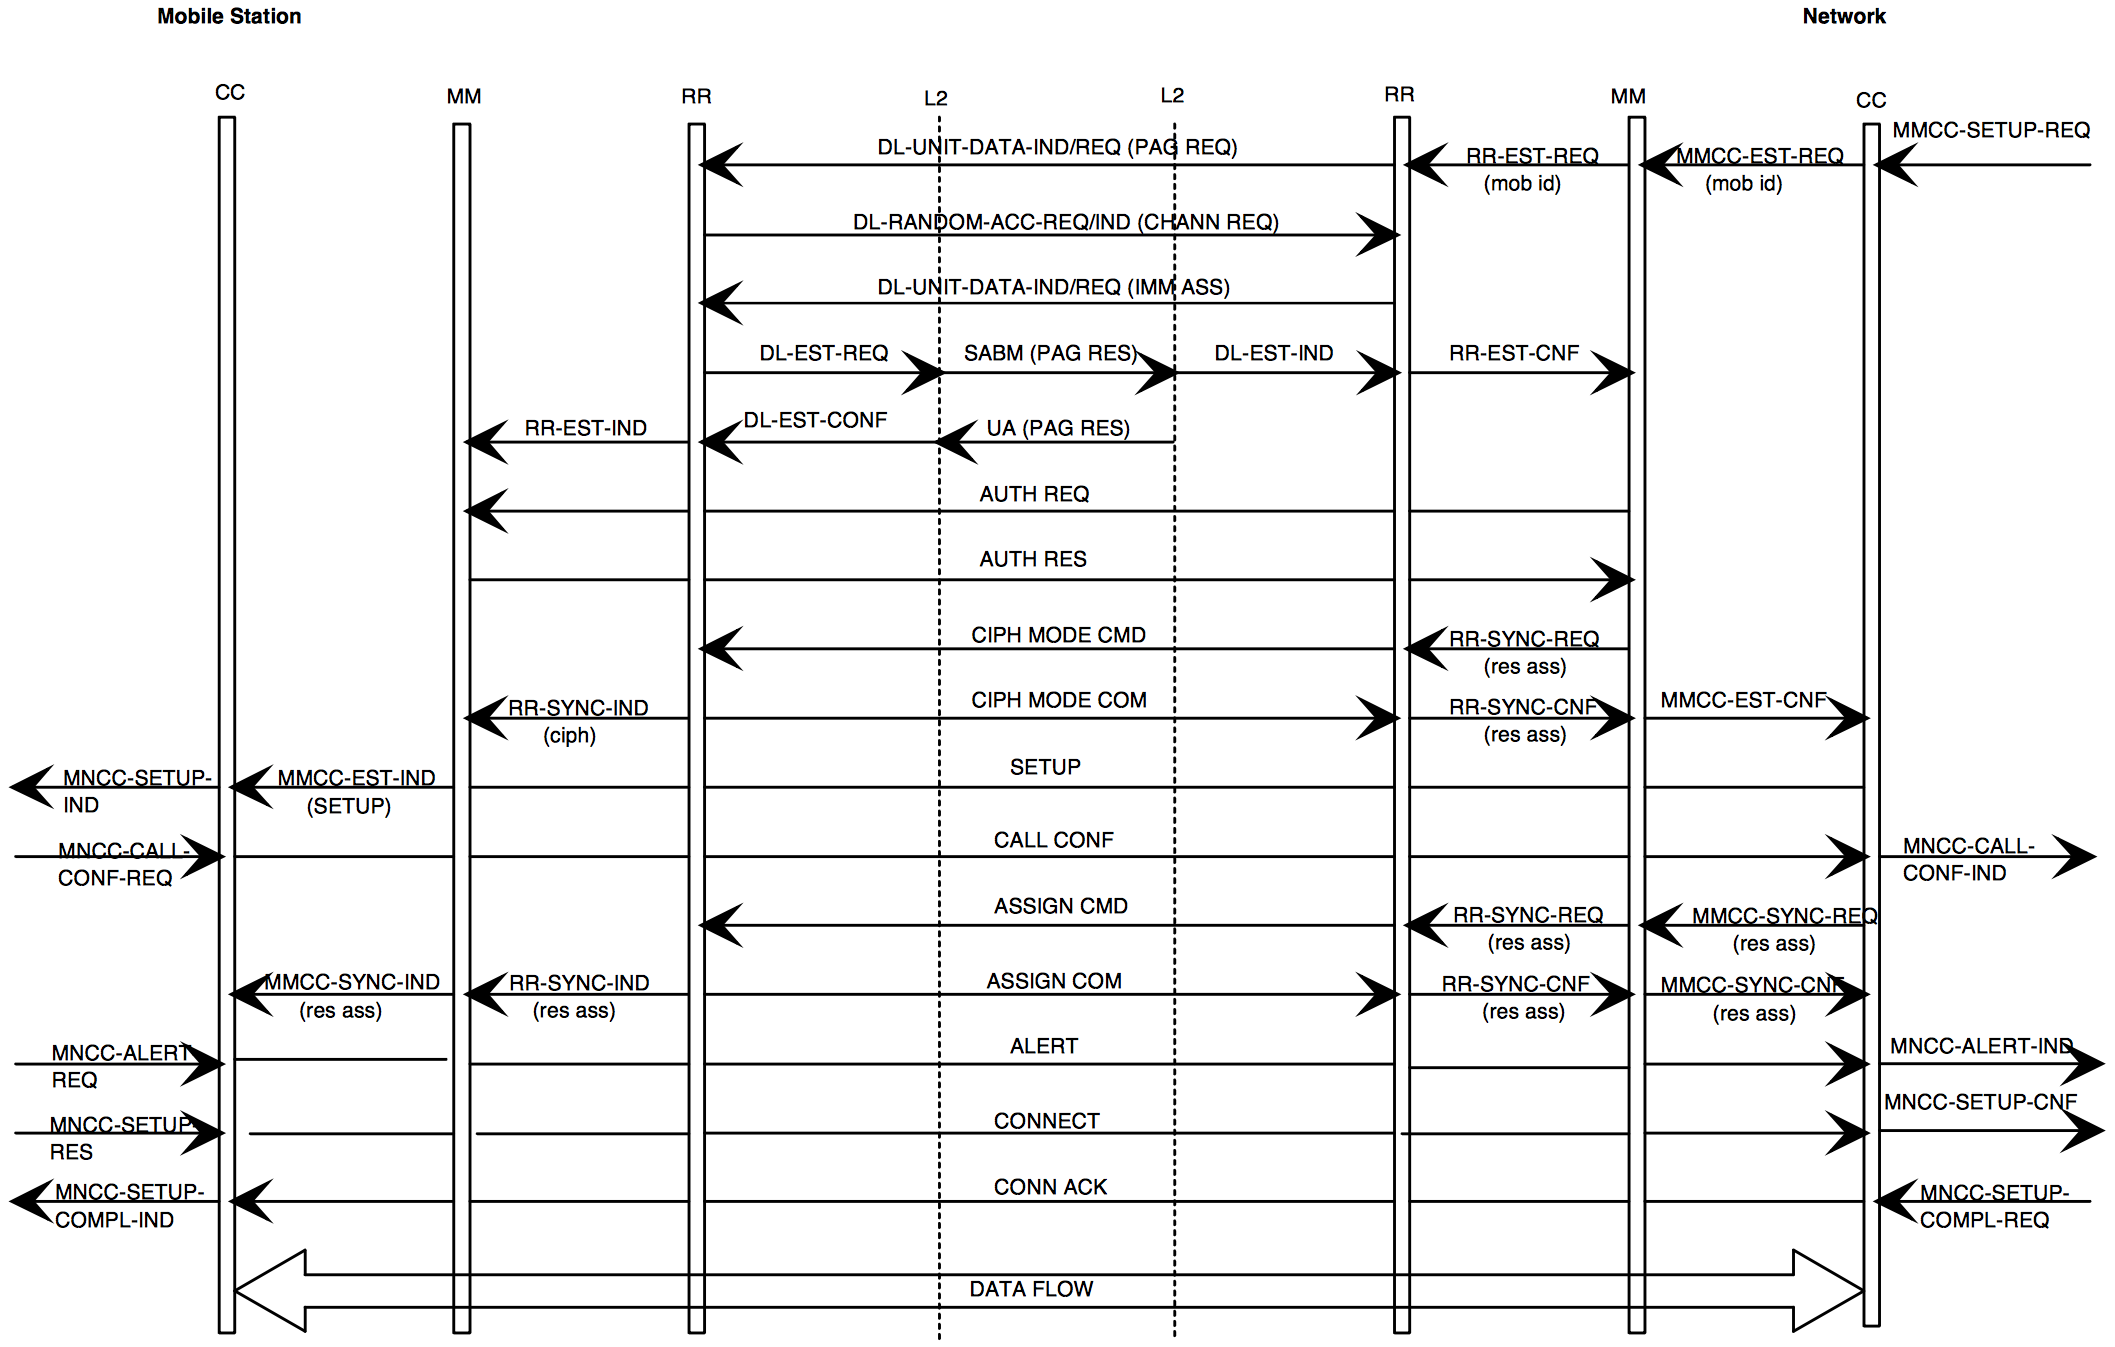
\includegraphics[width=\textwidth]{flow_mtc_setup}
        \caption{Mobile Terminated Call
        setup~\cite[p.~115]{3gpp_ts_2014-6}}
        \label{fig:flow_mtc_setup}
      \end{figure}

      \begin{figure}[h]
        \centering
        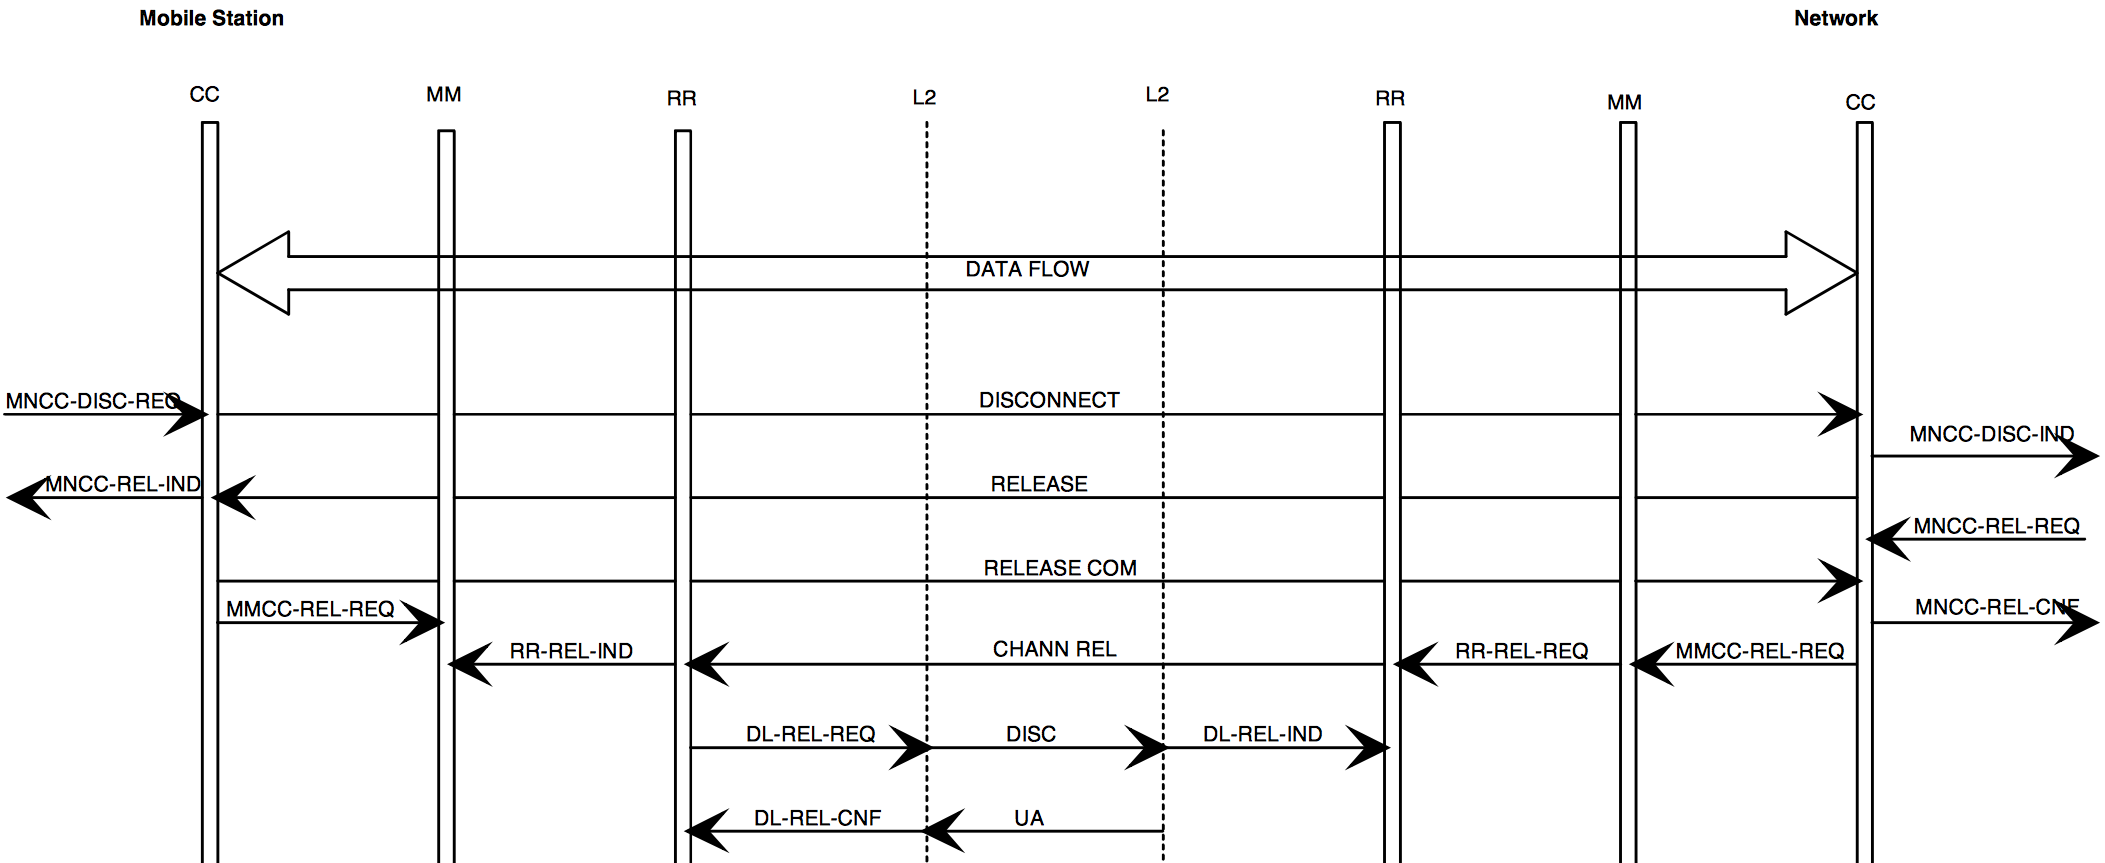
\includegraphics[width=\textwidth]{flow_moc_release}
        \caption{Mobile Originating Call
        release~\cite[p.~116]{3gpp_ts_2014-6}}
        \label{fig:flow_moc_release}
      \end{figure}

      \begin{figure}[h]
        \centering
        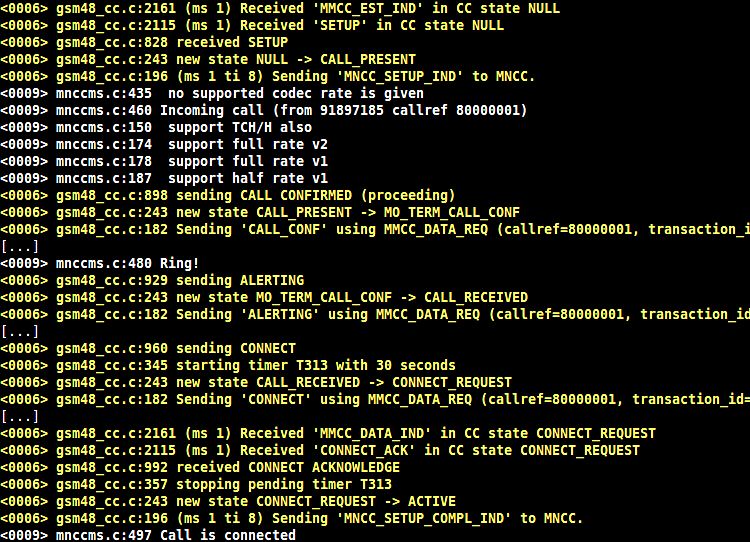
\includegraphics[width=\textwidth]{mobile_mtc_setup}
        \caption{Mobile Terminated Call
          setup in \prog{mobile}~\cite[p.~115]{3gpp_ts_2014-6}}
        \label{fig:mobile_mtc_setup}
      \end{figure}

      \begin{figure}[h]
        \centering
        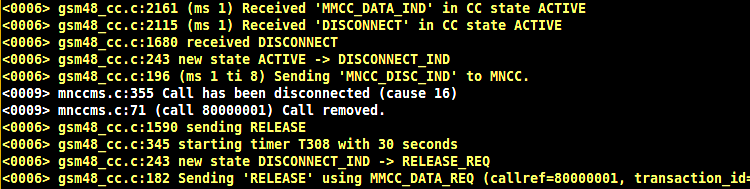
\includegraphics[width=\textwidth]{mobile_mtc_release}
        \caption{Mobile Terminating Call
        release in \prog{mobile}~\cite[p.~116]{3gpp_ts_2014-6}}
        \label{fig:mobile_mtc_release}
      \end{figure}

      \iffalse
  \section{OsmocomBB applications}

    The \prog{mobile} application was used along this chapter to
    demonstrate the various procedures of \gls{gsm}. It is not the only
    application available.


    The point of this chapter is too link the specifications with the
    \proj{OsmocomBB} project. To do so, various applications of the
    project will be introduced. The last one, \prog{mobile}, will be
    used to 



    using osmocombb applications
      ~\cite{osmocombb_applications}
      ~\cite{osmocombb_overview}

    \subsection{Osmocon}

    \iffalse
      \begin{figure}[h]
        \centering
        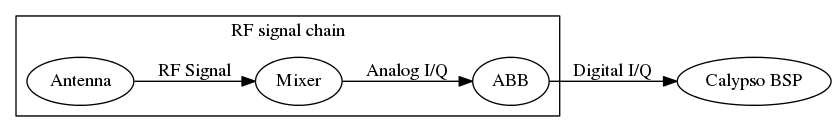
\includegraphics[width=\textwidth]{osmocombb_arch1}
        \caption{~\cite{osmocombb_overview}}
        \label{fig:osmocombb_arch1}
      \end{figure}

      \begin{figure}[h]
        \centering
        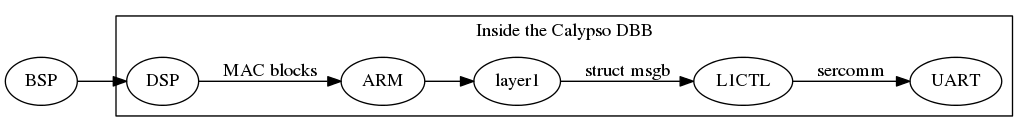
\includegraphics[width=\textwidth]{osmocombb_arch2}
        \caption{~\cite{osmocombb_overview}}
        \label{fig:osmocombb_arch2}
      \end{figure}

      \begin{figure}[h]
        \centering
        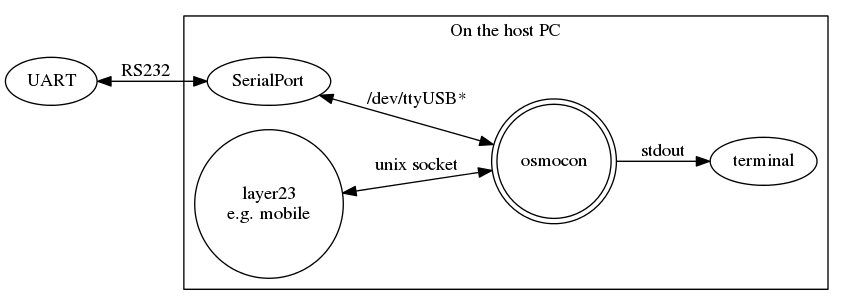
\includegraphics[width=\textwidth]{osmocombb_arch3}
        \caption{~\cite{osmocombb_overview}}
        \label{fig:osmocombb_arch3}
      \end{figure}
      \fi

      \begin{figure}[h]
        \centering
        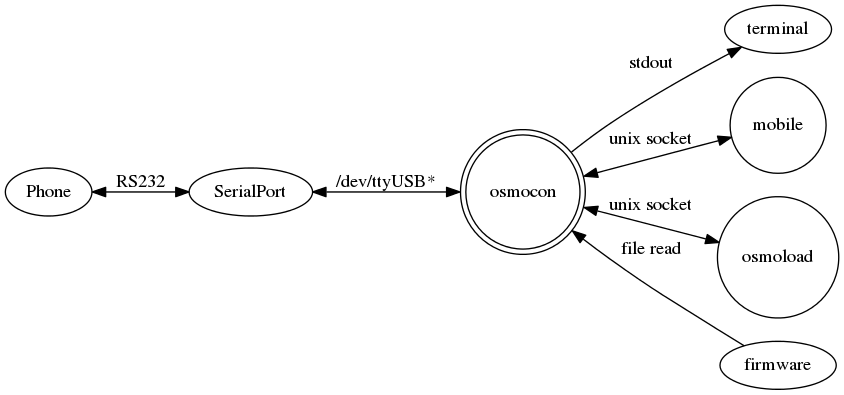
\includegraphics[width=\textwidth]{osmocon}
        \caption{~\cite{osmocombb_osmocon}}
        \label{fig:osmocon}
      \end{figure}

    \subsection{\prog{cell\_log}}

    \iffalse
       The cell_log application scans through valid available carrier
       frequencies, attempts to sync to them and dumps information
       gathered from the BCCH.

       It is usually used to create a list of used ARFCNs and
       information such as their reception levels, MNC, MCC, and System
       Information. 
       \fi

       Scans the bcch.

      \begin{figure}[h]
        \centering
        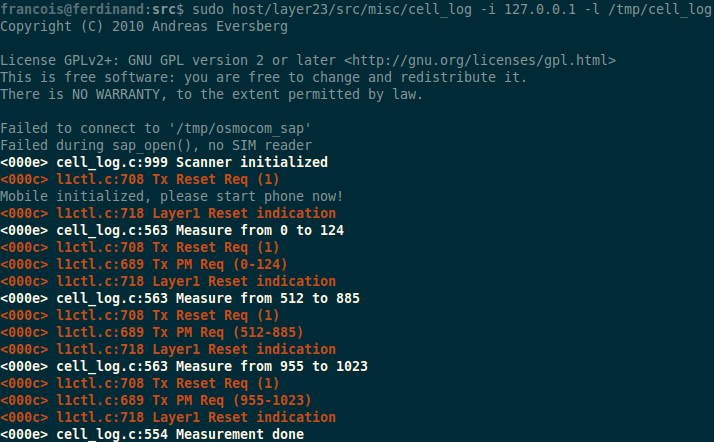
\includegraphics[width=\textwidth]{app_cell_log}
        \caption{The \prog{cell\_log} application first scans through
        all the ARFCNs, and measures their power level.}
        \label{fig:app_cell_log}
      \end{figure}

      \begin{figure}[h]
        \centering
        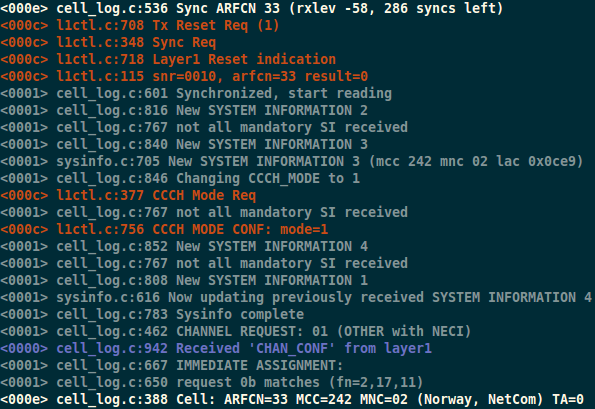
\includegraphics[width=\textwidth]{app_cell_log1}
        \caption{Then, starting with the best received ARFCN, it
          synchronizes with the cell, and gather information from the
          BCCH. Finally, it sends a Channel Request message and listens
          to the Immediate Assignment message to determine the Timing
          Advance parameter.}
        \label{fig:app_cell_log1}
      \end{figure}

      \begin{lstlisting}[language=C, numbers=left,
      basicstyle=\footnotesize, breaklines=true, frame=single]
        [sysinfo]
        arfcn 33
        time 1433681748
        bsic 5,7
        rxlev -56
        si1 55 06 19 00 00 00 00 00 00 00 00 00 00 00 01 10 00 00 00 a5 00 00 2b
        si2 59 06 1a 00 00 00 00 00 00 00 00 00 00 94 04 32 98 18 d0 df a5 00 00
        si3 49 06 1b fa fb 42 f2 20 0c e9 c8 02 28 24 45 40 a5 00 00 80 00 01 1b
        si4 31 06 1c 42 f2 20 0c e9 45 40 a5 00 00 80 00 4b 2b 2b 2b 2b 2b 2b 2b
        ta 0
        \end{lstlisting}
    
    \subsection{\prog{ccch\_scan}}

    \iffalse
    The ccch_scan application can sync to a carrier ARFCN and logs power
    measurement and CCCH information (paging requests and Immediate
    Assignments). 
    \fi

      Scans the ccch.

      \begin{figure}[h]
        \centering
        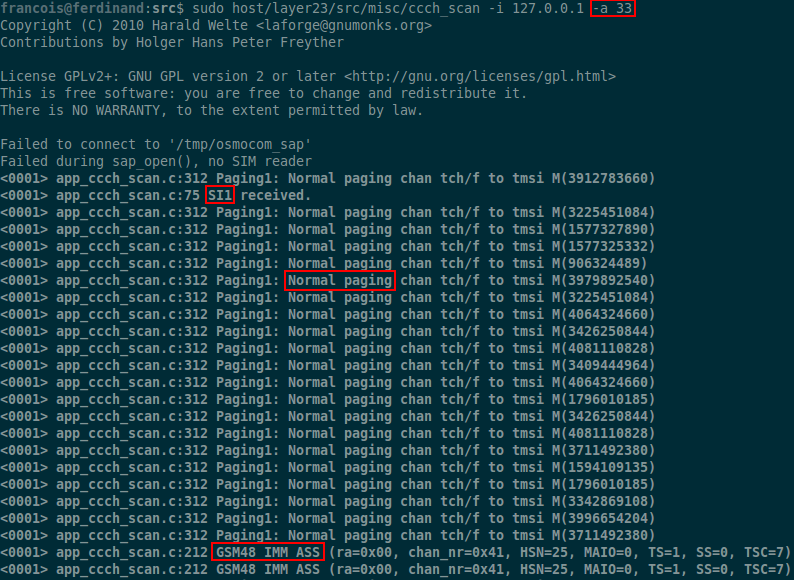
\includegraphics[width=\textwidth]{app_ccch_scan}
        \caption{This application scans the CCCH of a given ARFCN. It
        first reads SI1 and SI3 to get the needed parameters, then it
      listens and displays the Paging Request messages on the PCH, and
    the Immediate Assignment messages on the AGCH.}
        \label{fig:app_ccch_scan}
      \end{figure}

    \subsection{\prog{mobile}}

    \iffalse
     mobile is the most sophisticated OsmocomBB application so far.

     It implements most of the behavior of a regular GSM telephone, but
     is extended in many ways with features interesting to researchers. 
     \fi

     \url{http://bb.osmocom.org/trac/wiki/mobile}


     \iffalse
      The mobile program is one of the various host (PC) based programs
      that you can use together with the layer1.*.bin firmware images
      inside the phone.

      mobile is the most sophisticated OsmocomBB application so far. It
      implements most of the behavior of a regular GSM telephone, but is
      extended in many ways with features interesting to researchers.

      Using mobile, you can e.g.

          perform cell (re)selection according to TS 03.22
              MM procedures like location updating, authentication,
              encryption
                  Establish MT and MO voice calls
                      Send and receive SMS
                          Perform supplementary services like USSD or
                          call forwarding
                              hook it up to a PBX 

                              In the spirit of all Osmocom projects, the
                              user interface of mobile is based on text
                              commands issued on the command line. 
    \fi


    \iffalse
      \begin{figure}[h]
        \centering
        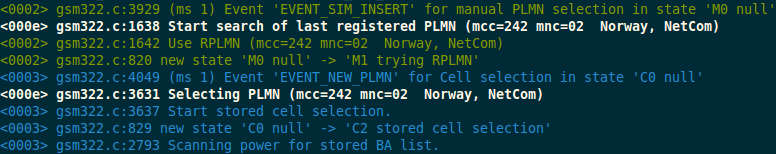
\includegraphics[width=\textwidth]{mobile_sim_insert}
        \caption{.}
        \label{fig:mobile_sim_insert}
      \end{figure}
      \begin{figure}[h]
        \centering
        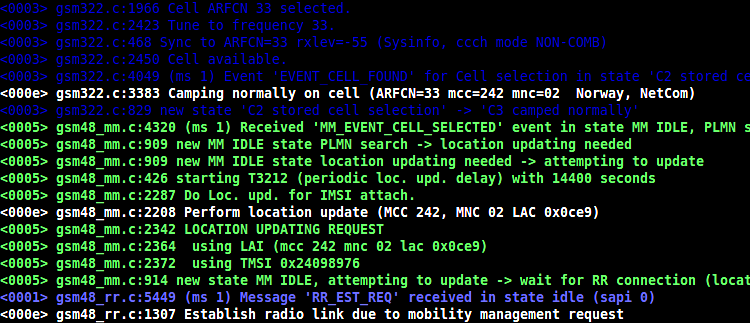
\includegraphics[width=\textwidth]{mobile_loc_up}
        \caption{.}
        \label{fig:mobile_loc_up}
      \end{figure}
      \begin{figure}[h]
        \centering
        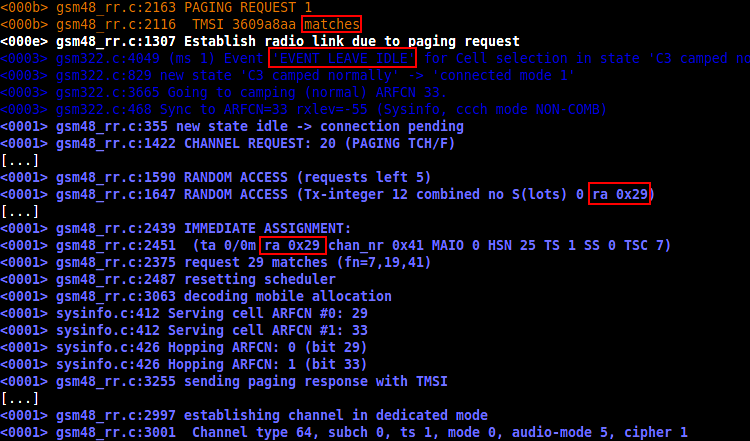
\includegraphics[width=\textwidth]{mobile_rach}
        \caption{.}
        \label{fig:mobile_rach}
      \end{figure}
      \begin{figure}[h]
        \centering
        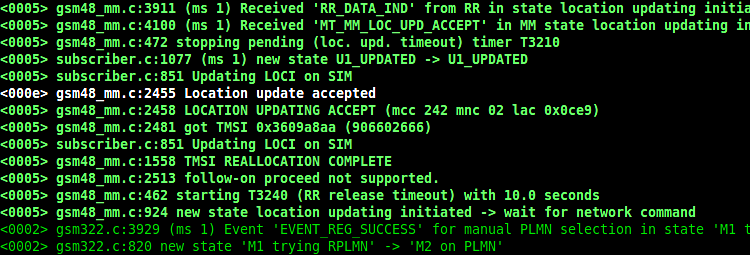
\includegraphics[width=\textwidth]{mobile_loc_acc}
        \caption{.}
        \label{fig:mobile_loc_acc}
      \end{figure}
      \begin{figure}[h]
        \centering
        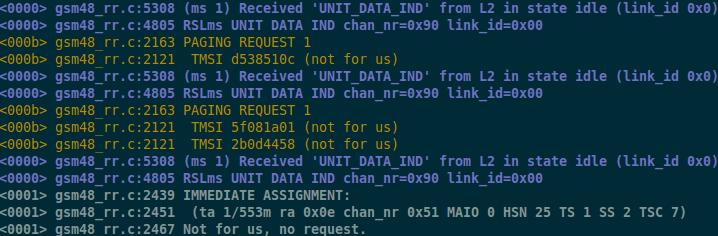
\includegraphics[width=\textwidth]{mobile_idle}
        \caption{.}
        \label{fig:mobile_idle}
      \end{figure}
      \begin{figure}[h]
        \centering
        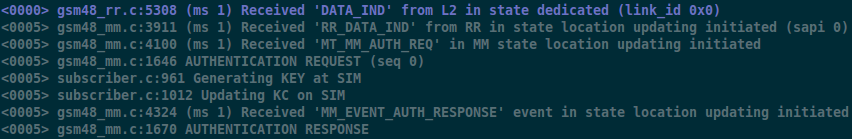
\includegraphics[width=\textwidth]{mobile_auth}
        \caption{.}
        \label{fig:mobile_auth}
      \end{figure}
      \begin{figure}[h]
        \centering
        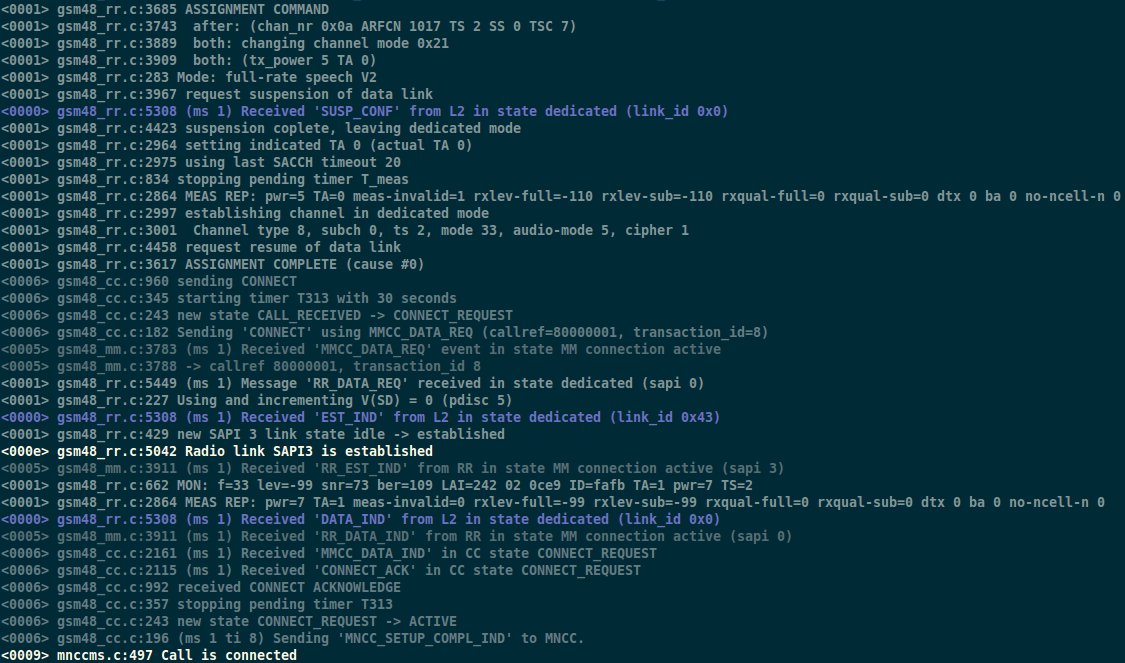
\includegraphics[width=\textwidth]{mobile_connect}
        \caption{.}
        \label{fig:mobile_connect}
      \end{figure}
      \begin{figure}[h]
        \centering
        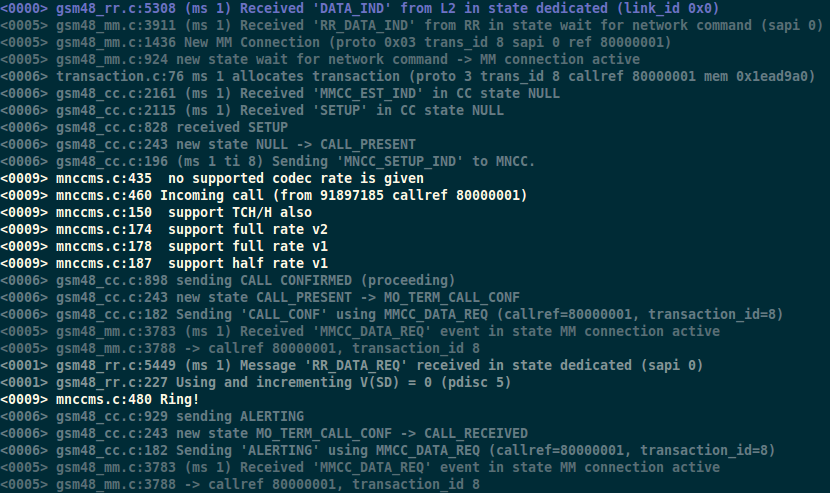
\includegraphics[width=\textwidth]{mobile_alerting}
        \caption{.}
        \label{fig:mobile_alerting}
      \end{figure}
      \begin{figure}[h]
        \centering
        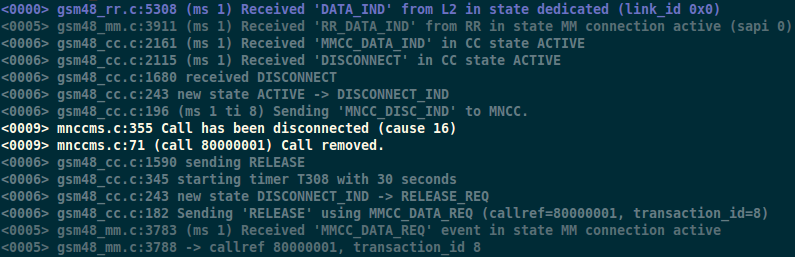
\includegraphics[width=\textwidth]{mobile_release}
        \caption{.}
        \label{fig:mobile_alerting}
      \end{figure}
      \begin{figure}[h]
        \centering
        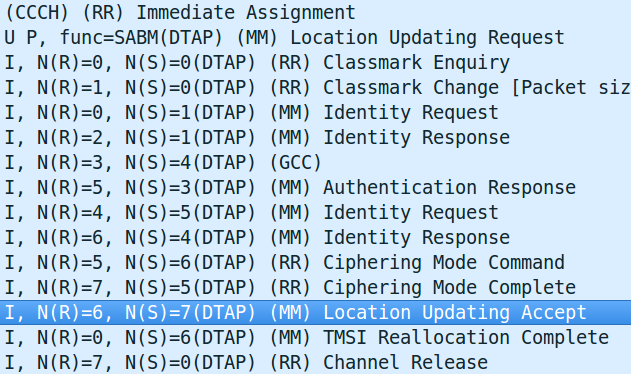
\includegraphics[width=\textwidth]{mobile_ws_lu}
        \caption{.}
        \label{fig:mobile_ws_lu}
      \end{figure}
      \begin{figure}[h]
        \centering
        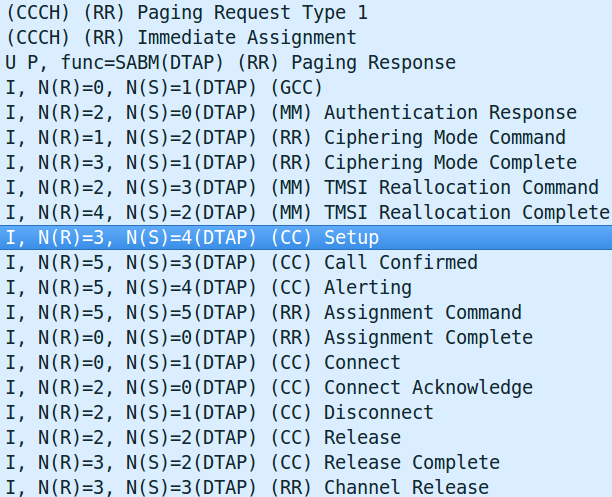
\includegraphics[width=\textwidth]{mobile_ws_mtc}
        \caption{.}
        \label{fig:mobile_ws_mtc}
      \end{figure}
      \begin{figure}[h]
        \centering
        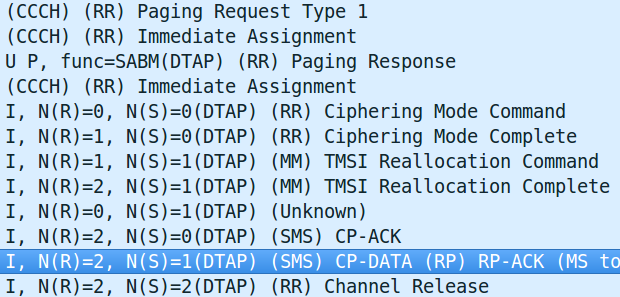
\includegraphics[width=\textwidth]{mobile_ws_mtsms}
        \caption{.}
        \label{fig:mobile_ws_mtsms}
      \end{figure}
      \fi
      \fi
